%% SW arkitektur: Deployment View

Deployment View skal illustrerer hvor hvilke lag af software der ligger på vores platforme. Devkit8000 kører Linux og har derfor flere softwarelag end PSoC'en.
 
\vspace{15 mm}

\begin{figure}[htbp] \centering
{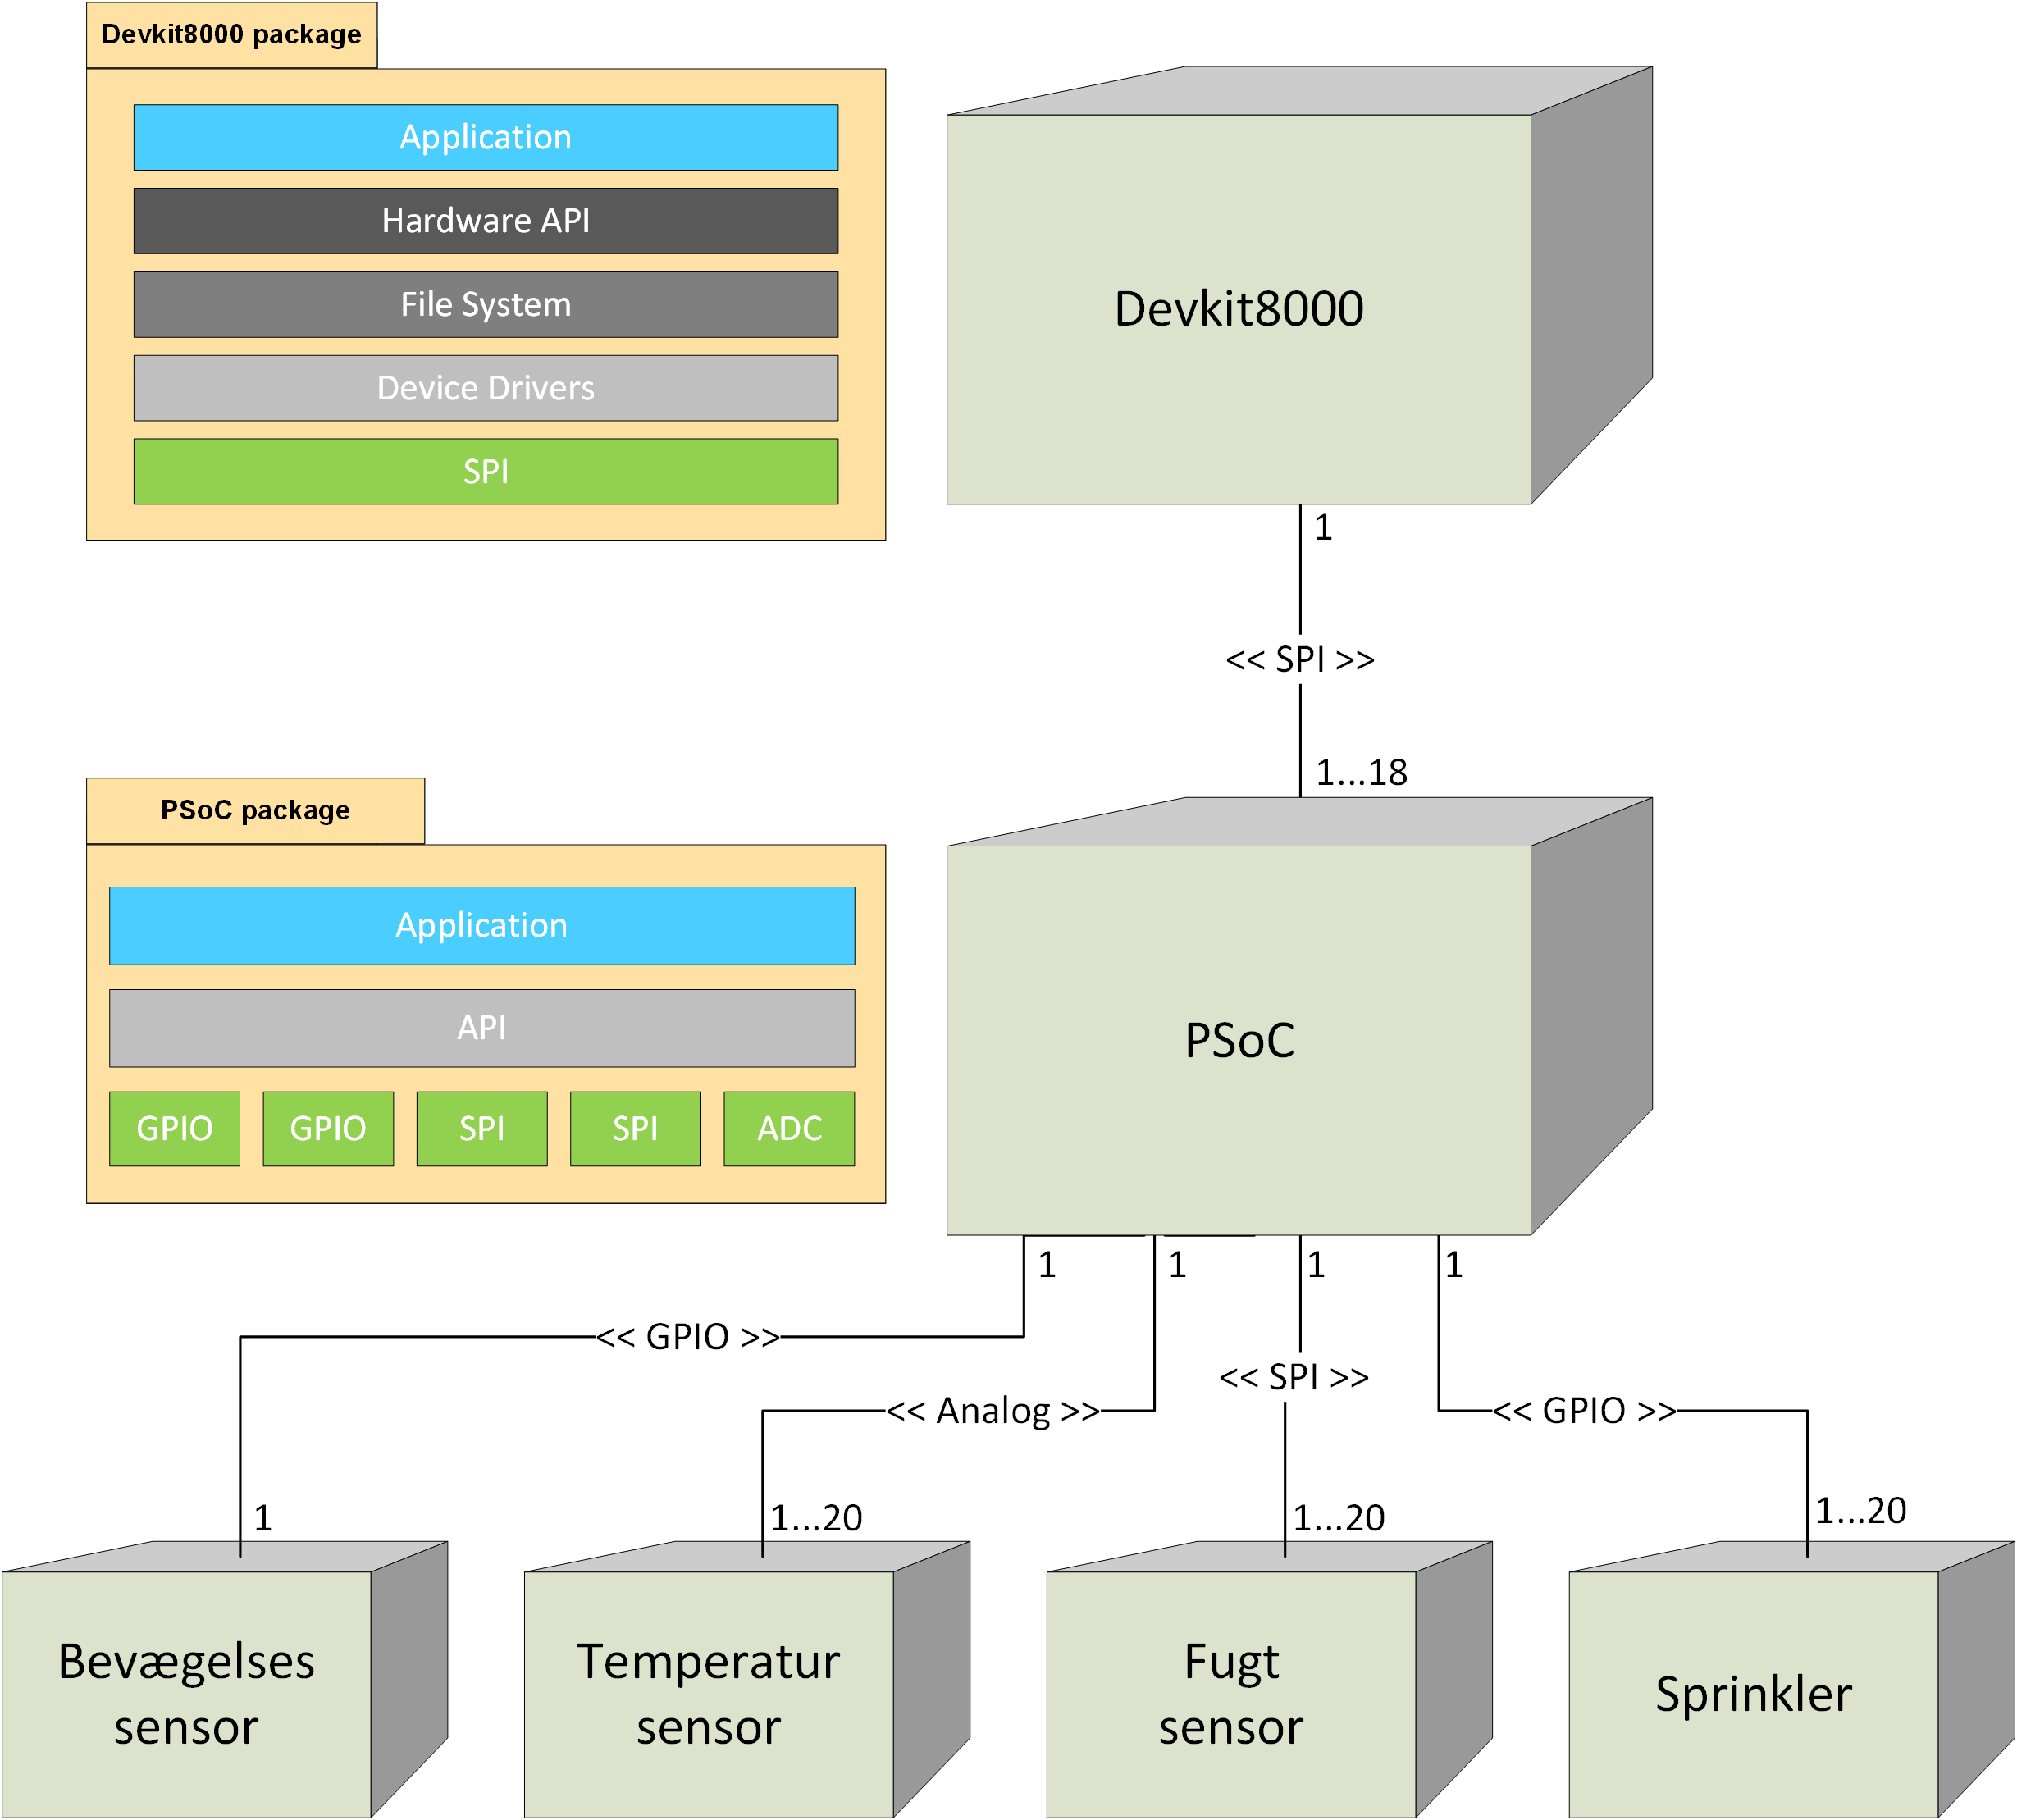
\includegraphics[scale=0.7]{filer/systemarkitektur/Deployment_model}}
\caption{Deployment model illustrerer de forskellige software og hardware(grønne) lag}
\label{fig:Deployment Model}
\end{figure}

Figur \ref{fig:Deployment Model} viser hvilke lag der er i de respektive pakker og hvor pakkerne hører til. \textit{File system} er en del af Linux systemet og ikke noget der skal implementeres.

\clearpage

\begin{figure}[!htbp] \centering
{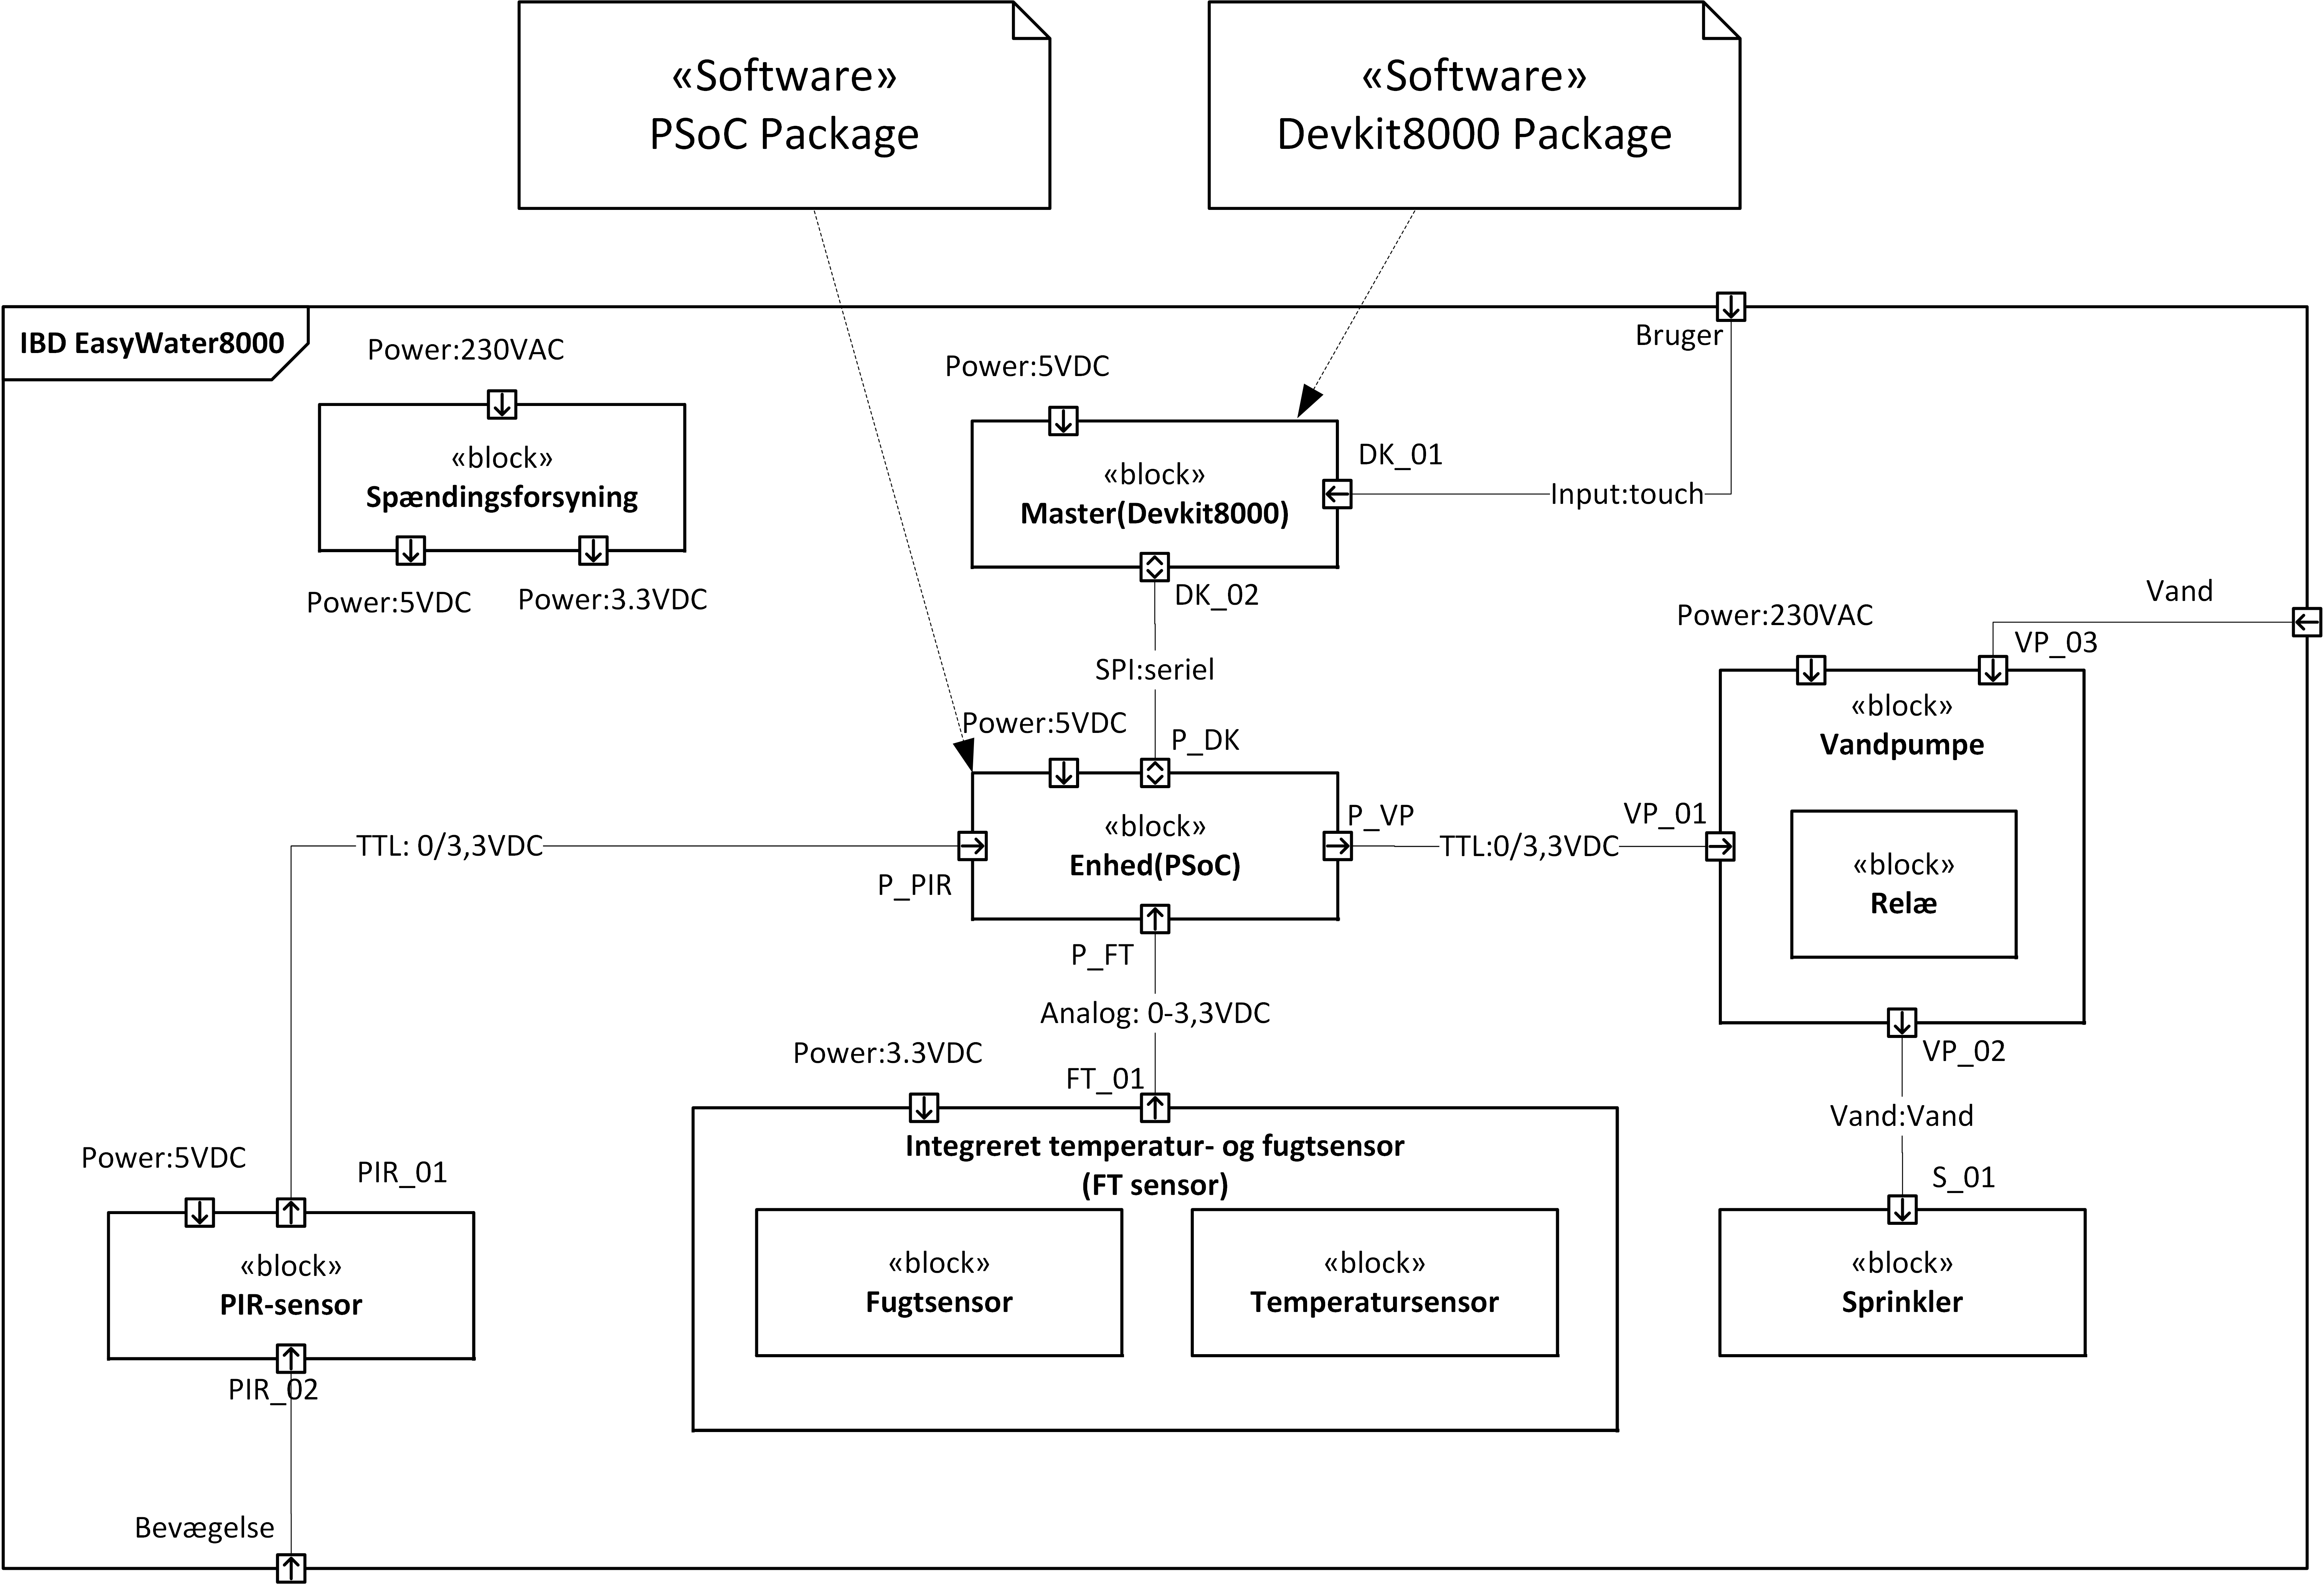
\includegraphics[scale=0.7]{filer/systemarkitektur/IBD_deployment}}
\caption{IBD med software packages}
\label{fig:IBD deployment}
\end{figure}

Figur \ref{fig:IBD deployment} viser pakkernes placering på det interne blokdiagram, så man kan se præcist hvor softwaren kommer til at ligge på hardwaren.